\section{Discussion} 
\label{sec:Discussion}

% \subsection{Matched features}
% In this section, we discuss matched features to investigate prediction
% performance on cross-domain defect prediction in detail.
% 
% \begin{figure}[t]
% 	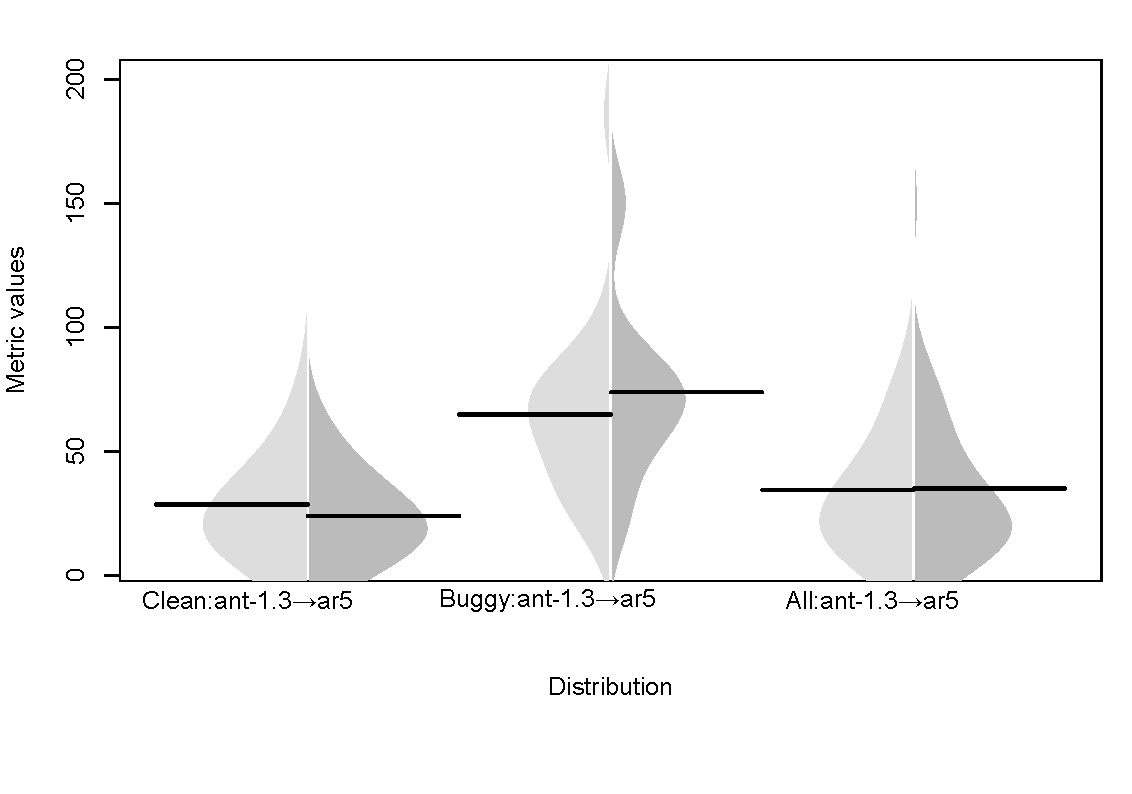
\includegraphics[width=\linewidth]{Figures/Result/best_dist.pdf}
% 	\caption{Feature value distribution of a matched feature from the
% 	prediction combination, ant-1.3$\Rightarrow$ar5, of AUC=0.938.}
% 	\label{fig:best_dist}
% \end{figure}
% 
% % A reason why ASAnalyzer can predict defects pretty well on cross-domain
% % settings is that most defect prediction metrics usually represent complexity of
% % source code and its change; it tends to be more buggy when the complexity is
% % higher.
% 
% In Figure~\ref{fig:best_dist}, we used beanplots~\cite{Beanplot08} to represent
% the feature value distribution of a matched feature in the prediction
% combination, ant-1.3$\Rightarrow$ar5, whose AUC is 0.938. The left side (light
% grey) of each beanplot shows distribution of buggy, clean, and all instances of
% source respectively, while the right side (dark grey) of each beanplot
% represents those of target. The horizontal black line represents an average
% value in each distribution. 
% 
% From Figure~\ref{fig:best_dist}, we can explain how ant-1.3$\Rightarrow$ar5 can
% have such a high AUC, 0.938. Suppose that a simple model predicts an instance as
% buggy when the feature value of the instance is more than 40 in case of
% Figure~\ref{fig:best_dist}. In both the source and target, approximately
% 70\% or more buggy and clean instances will be predicted correctly. In
% Figure~\ref{fig:best_dist}, the matched source and target features in
% ant-1.3$\Rightarrow$ar5 are the response for class (RFC: number of methods
% invoked by a class~\cite{Chidamber94}) and the number of unique operands
% (unique\_operands), respectively. The RFC and unique\_operands are not the same
% features. However, they have similar distribution as shown in
% Figure~\ref{fig:best_dist}. As we explained in Section~\ref{sec:Approach},
% typical defect prediction metrics (features) have a tendency that a higher
% complexity causes more buggy- proneness. The matched features
% follow this tendency very well so that the model using the matched features
% could achieve such a high AUC (0.938).
%but related; both features can be a factor contributing to how long and complex
% the source code is. In ar5, there is a more related feature such as comment\_loc. However, they are not actually matched since they have different distribution in terms of mean and standard deviation.

% \begin{figure}[t]
% 	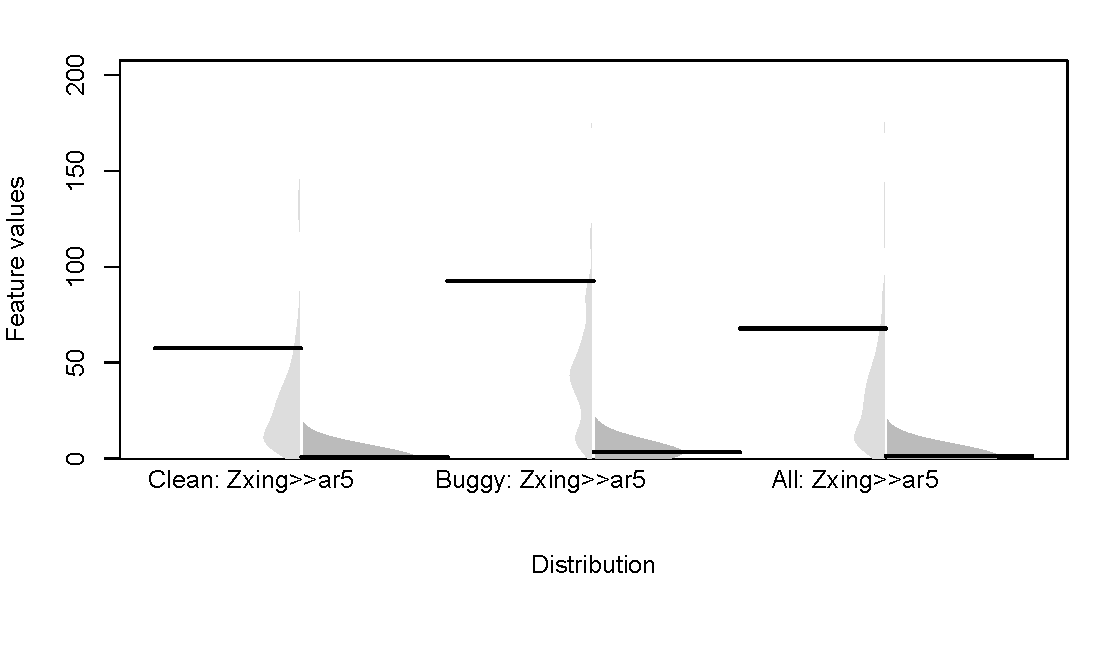
\includegraphics[width=\linewidth]{Figures/Result/beanplot_manual_matching.pdf}
% 	\caption{Feature value distribution of a manually matched feature (attribute)
% 	from the prediction combination, Zxing$\Rightarrow$ar5, of AUC=0.57.}
% 	\label{fig:manual_dist}
% \end{figure}
% 
% Each project
% may have different feature distributions even in projects with the same features
% since project characteristics can be made different by many other external
% environments such as the number of developers, product types, intended audiences, and so on.~\cite{Zimmermann09}.
% 
% Figure~\ref{fig:manual_dist} shows the feature value distribution of a
% manually matched feature of the prediction combination, Zxing$\Rightarrow$ar5, with AUC=0.57. The
% source and target features are CountLineCode and code-and-commend-loc
% respectively. Both features measure lines of code and comments, however their
% distributions are too different as seen in Figure~\ref{fig:manual_dist}. This
% is why cross-project prediction on projects with the same feature space is
% still a challenging issue~\cite{He12, Turhan09,Zimmermann09}. Thus, we tried to
% match features, which have similar distribution in a mechanical way to compare
% statistical parameters such as mean and standard deviation and observed
% many better prediction (Win) performance results as shown in
% Table~\ref{tab:win_results}.

\subsection{Why Matched Metric Works?}
\label{sec:why}
\begin{figure}[t]
	\centering
	\vspace{0.5mm}
	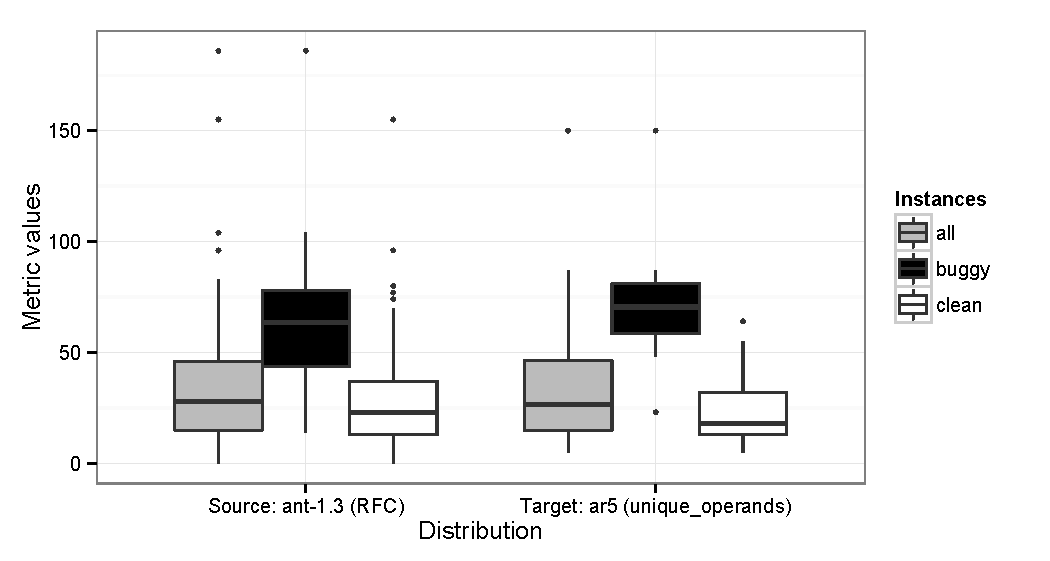
\includegraphics[width=\linewidth]{Figures/Result/best_dist_bplot.pdf}
	\caption{Distribution of metrics (matching score=0.91)
	from ant-1.3$\Rightarrow$ar5 (AUC=0.946).}
	\label{fig:best_dist}
\end{figure}

In Figure~\ref{fig:best_dist}, we use box plots to represent
distributions of matched metrics.
% the feature value distribution of
% a matched feature in the prediction combination, ant-1.3$\Rightarrow$ar5, whose AUC is 0.938.
The gray, black, and white box plots shows distributions of matched metrics in
all, buggy, and clean instances respectively. The three box plots on the
left-hand side represent distributions of a source metric while the three
box plots on the right-hand side represent those of a target metric. The
bottom and top of the boxes represent the first and third quartiles
respectively.
The solid horizontal line in a box represents the median value in each distribution. 
Black points in the figure are outliers.

Figure~\ref{fig:best_dist} explains how the prediction
combination of ant-1.3$\Rightarrow$ar5 can have a high AUC, 0.946. Suppose
that a simple model predicts that an instance is buggy when the metric value of
the instance is more than 40 in the case of Figure~\ref{fig:best_dist}. In both
datasets, approximately 75\% or more buggy and clean instances will be
predicted correctly. In Figure~\ref{fig:best_dist}, the matched metrics in
ant-1.3$\Rightarrow$ar5 are the response for class ({\em RFC}: number of methods
invoked by a class)~\cite{Chidamber94} and the number of unique operands ({\em
unique\_operands})~\cite{Halstead77}, respectively. The {\em RFC} and {\em
unique\_operands} are not the same metric so it might look like an arbitrary
matching. However, they are matched based on their similar distributions as
shown in Figure~\ref{fig:best_dist}. Typical defect prediction metrics have
tendencies in which higher complexity causes more
bug-proneness~\cite{DAmbros12,Menzies07,Rahman13}. In
Figure~\ref{fig:best_dist}, instances with higher values of {\em RFC} and {\em
unique\_operands} have the tendency to be more bug-prone. For this reason, the
model using the matched metrics could achieve such a high AUC (0.938). We could
observe this bug-prone tendency in other Win results. Since matching metrics is
based on similarity of source and target metric distributions, HDP also
addresses several issues related to a dataset shift such as the covariate shift
and domain shift discussed by Turhan~\cite{Turhan12}.

Some prediction combinations have Loss results in
Table~\ref{tab:win_results}. We investigated matched metrics in these
prediction combinations. In velocity-1.4 of Table~\ref{tab:win_results}, all
results are Loss. Thus, as a representative loss result, we discuss the
prediction combination, Safe$\Rightarrow$velocity-1.4, whose AUC is 0.391.

\begin{figure}[t]
	\centering
	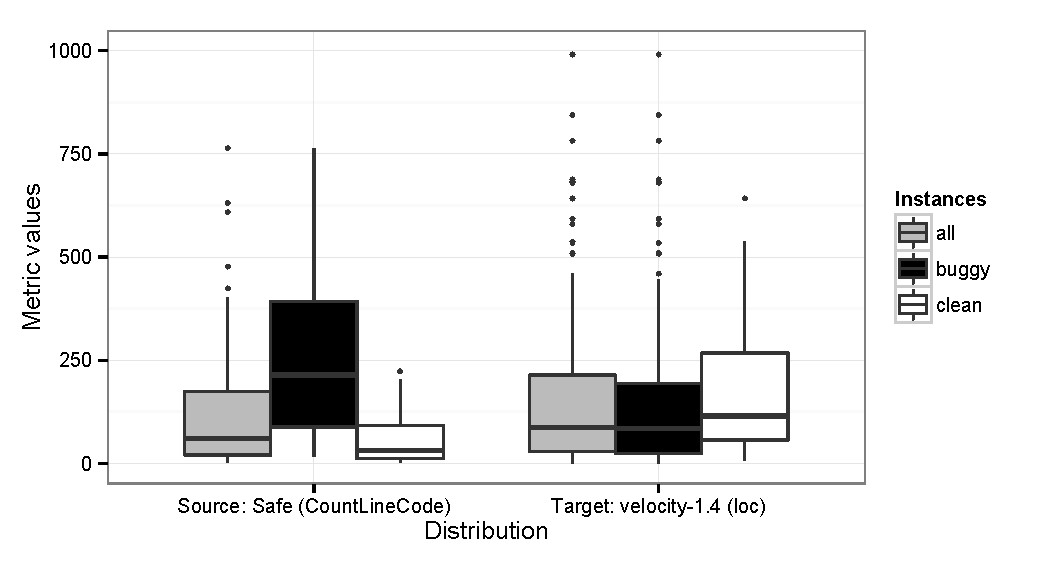
\includegraphics[width=\linewidth]{Figures/Result/loss_dist_bplot.pdf}
	\caption{Distribution of metrics (matching score=0.45)
	from Safe$\Rightarrow$velocity-1.4 (AUC=0.391).}
	\label{fig:loss_dist}
\end{figure}

As observed, Loss results were usually caused by different tendencies of
bug-proneness between source and target metrics. Figure~\ref{fig:loss_dist}
shows how the bug-prone tendencies of source and target metrics are different.
Interestingly, the matched source and target metric by the KSAnalyzer is the
same as {\em LOC} ({\em CountLineCode} and {\em loc}) in both.
As we observe in the figure, the median of buggy instance values of the
source metric is higher than that of clean instances in that the more {\em LOC}
implies the higher bug-proneness in the case of Safe. However, the median of
buggy instance values in a target metric is lower than that of clean instance values
in that the less {\em LOC} implies the higher bug-proneness in
velocity-1.4. This inconsistent tendency of
bug-proneness between the source and target metrics could degrade the
prediction performance although they are the same metric.

We regard the matching that has an inconsistent bug-prone tendency between
source and target metrics as a noisy metric matching.
% This implies the target
% feature does not follow the tendency that a higher complexity causes more bug-proneness.
% The target feature worked as noise when the model predicted
% defects in velocity-1.4. 
We could observe this kind of noisy metric matching in
prediction combinations in other Loss results.

However, it is very challenging to filter out the noisy metric matching since we
cannot know labels of target instances in
advance. If we could design a filter for the noisy metric matching, the Loss
results would be minimized. Thus, designing a new filter to mitigate these Loss
results is an interesting problem to address. Investigating this new filter
for the noisy metric matching will remain as future work.

Figure~\ref{fig:loss_dist} also explains why CPDP-CM did not show reasonable
prediction performance. Although the matched metrics are same
as {\em LOC}, its bug-prone tendency is inconsistent. Thus, this matching using
the common metric was noisy and was not helpful for building a prediction model.

We also investigated whether the performance of HDP can be affected by the
size of a target dataset. If the size of a target dataset gets smaller, it
might be difficult to precisely compute distribution similarity between source
and target metrics. As in Table~\ref{tab:datasets}, the sizes of datasets
vary from 36 (ar5) and 1862 (ML), and the results of HDP in
Table~\ref{tab:win_results} also vary. We could not find any relation between
the size of a target and the prediction performance. In ar5 of Table~\ref{tab:win_results}, 14 out of 18 predictions led to Win results,
while in ML, all six predictions led to Loss results. In velocity-1.4
that has a relatively small number (196) of instances compared to other
datasets, all three predictions had Loss results. However, tomcat that is of a
bigger size (858) than velocity-1.4 had only Win results. As discussed, the
prediction performance of HDP is dependent on the bug-prone tendencies of
the matched metrics. If the matched metrics are consistent in terms of the
bug-prone tendency, HDP can lead to promising results regardless of
the size of the target dataset.
% The DM filter could not remove
% this matched feature since the modality of all instances in both source and
% target is still similar. Without knowing labels of target instances, it is
% difficult to filter out this case. Other Loss results also have similar
% observations. Designing new filters for these Loss results is a challenging
% issue since we cannot know distribution of clean and buggy instances of target in
% advance. Investigating new filters for these patterns remains as future work.



% The pc4 in Table~\ref{tab:win_results} also have many Loss results.
% However, note that pc4 still have very high AUC values, 0.899 and 0.70,
% respectively, The AUC value of 0.70 is considered as a promising result in defect prediction~\cite{Giger12, Lessmann08}. The reason for Loss results
% of pc1 and pc3 is that within-results in AUC are already very high, 0.78 and
% 0.79, respectively.


%\TODO{Guidelines or suggestions on cross-domain defect prediction?}

\subsection{Performance in Different Metric Selections}

\begin{table}[!t]
%\small
\scriptsize
\centering
\caption{Prediction performance (a
median AUC and \% of Win) in different metric selections.
% Between within- and
% cross-results by
% analyzers, outperforming results with statistical significance
% (Wilcoxon signed-rank, p$<$0.05) is bold-faced. Between cross-results using
% common features and by analyzers, outperforming results with
% statistical significance (Wilcoxon signed-rank, p$<$0.05) is underlined.}
}
\label{tab:various_fs}
%\setlength{\tabcolsep}{5pt}
%\setlength{\extrarowheight}{1.5pt}
\begin{tabular}{|@{}c@{}||c@{ }|@{}c@{}||c@{ }|@{}c@{}||c@{ }|@{}c@{}||c|}
%\begin{tabular}{|c||C|C||C|C||C|C||C|}
\hline
\multirow{3}{*}{\bf{Approach}}
&\multicolumn{6}{@{ }c@{ }||}{\bf Against}
&\multirow{2}{*}{\specialcell{\bf{HDP}}}
\\\cline{2-7}
&\multicolumn{2}{@{ }c@{ }||}{\specialcell{\bf{WPDP}}}
&\multicolumn{2}{@{ }c@{
}||}{\specialcell{\bf{CPDP-CM}}}
&\multicolumn{2}{@{ }c@{ }||}{\specialcell{\bf{CPDP-IFS}}}
&
\\
\cline{2-8}
& \bf{AUC}
& \bf{Win\%}
& \bf{AUC}  
& \bf{Win\%}
& \bf{AUC}  
& \bf{Win\%}
& \bf{AUC}  
\\
\hline
\hline
Gain Ratio	& 0.657 &63.7\%	&0.645 &63.2\% &0.536 &80.2\% &0.720	\\ \hline
Chi-Square	& 0.657 &64.7\%	&0.651 &66.4\% &0.556 &82.3\% &0.727  \\ \hline
Significance& 0.657 &66.2\%	&0.636 &66.2\% &0.553 &82.0\% &0.724  \\ \hline
Relief-F		& 0.670 &57.0\%	&0.657 &63.1\% &0.543 &80.5\% &0.709	\\ \hline
None			& 0.657 &47.3\%	&0.624 &50.3\% &0.536 &66.3\% &0.663	\\ \hline
\end{tabular}
\end{table}

Table~\ref{tab:various_fs} shows prediction results on various metric selection approaches
including with no metric selection (`None'). We compare the median AUCs of
the HDP results by KSAnalyzer with the cutoff of 0.05 to those of WPDP, CPDP-CM,
or CPDP-IFS, and report \% of Win results.

Overall, we could observe metric selection to be helpful in improving
prediction models in terms of AUC. When applying metric selection, the Win results
account for more than about 63\% in most cases against WPDP and CPDP-CM. Against
CPDP-IFS, the Win results of HDP account for more than 80\% after appying the
metric selection approaches. This implies that the metric selection approaches
can remove irrelevant metrics to build a better prediction model. In addition, this result confirms
the previous studies that we can build prediction models better than or
comparable to WPDP models with even a few key metrics~\cite{Gao11, He14subset}.
However, the percentages of Win results in `None' were lower than those in
applying metric selection. Among metric selection approaches, `Chi-Square' and
`Significance' based approaches lead to the best performance in terms of the
percentage of the Win results (64.7\%-66.2\%) against WPDP.

\subsection{Performance in Various Analyzers}

% \begin{table*}[t]
% \scriptsize
% \centering
% \caption{Prediction performance in other analyzers with the matching
% score cutoff thresholds, 0.05 and 0.90. Significance attribute selection is used
% for metric selection.
% % Between within- and
% % cross-results by
% % analyzers, outperforming results with statistical significance
% % (Wilcoxon signed-rank, p$<$0.05) is bold-faced. Between cross-results using
% % common features and by analyzers, outperforming results with
% % statistical significance (Wilcoxon signed-rank, p$<$0.05) is underlined.}
% }
% \label{tab:other_analyzers}
% %\setlength{\tabcolsep}{5pt}
% %\setlength{\extrarowheight}{1.5pt}
% %\begin{tabular}{|@{ }c@{ }|@{ }c@{ }||@{ }c@{ }||@{ }c@{ }|@{ }c@{ }|@{ }c@{
% %}||@{ }c@{ }||@{ }c@{ }|@{ }c@{ }|@{ }c@{ }||@{ }c@{ }||@{ }c@{ }|}
% \begin{tabular}{|c|c||c|c|c|c||c|c|c|c||c||c|}
% \hline
% \multirow{2}{*}{\specialcell{\bf{Analyzer}}}
% &\multirow{2}{*}{\specialcell{\bf{Threshold}}}
% &\multicolumn{4}{c||}{\textbf{Against WPDP}}
% &\multicolumn{4}{c||}{\specialcell{\bf{Against CPDP}\\\bf{using Common Metrics}}}
% &\specialcell{\bf{HDP by\\analyzers}}
% &\multirow{2}{*}{\specialcell{\bf{Target}\\\bf{Coverage}}}
% \\\cline{3-11}
% &
% & \bf{AUC}
% & \bf{Win\%}
% & \bf{Tie\%}
% & \bf{Loss\%}
% & \bf{AUC} 
% & \bf{Win\%}
% & \bf{Tie\%}
% & \bf{Loss\%}
% & \bf{AUC}
% & 
% \\
% \hline
% \hline
% %PAnalyzer& 0.00 & \bf{0.684}	& \underline{0.640}	& 0.606 & 100\% \\ \hline 
% PAnalyzer& 0.05 & \bf{0.684} & 30.3\% & 3.0\% & 66.7\%
% &\underline{0.640} & 45.1\% & 2.2\% & 52.7\%
% & 0.617 & 100\%
% \\
% \hline PAnalyzer& 0.90  & 0.657 & 54.2\% & 2.4\% & 43.4\%
% &0.622 & 65.1\% & 1.2\% & 33.7\%
% & \underline{0.692} & 96\% \\
% \hline
% \hline
% \hline
% 
% %KSAnalyzer & 0.00 & 0.670 &	0.637	& \underline{0.669} & 100\% \\ \hline 
% KSAnalyzer & 0.05 & 0.657 & 66.2\% & 1.4\% & 32.4\% 
% &0.636 & 66.2\% & 6.3\% & 27.5\% 
% &\underline{\bf{0.724}} &100\% \\
% \hline KSAnalyzer& 0.90  & 0.657 & 100\% & 0.0\% & 0.0\%
% &0.761 & 71.4\% & 0.0\% & 28.6\%
% &\bf{0.852}&21\% \\ \hline
% \hline
% \hline
% 
% %SCoAnalyzer & 0.00 & \bf{0.684}	&\underline{0.640}	&0.517 & 100\% \\ \hline 
% SCoAnalyzer & 0.05 & \bf{0.684} & 28.5\% & 1.7\% & 69.8\%
% &\underline{0.640} & 37.3\% & 3.5\% & 59.2\%
% &0.542 & 100\%
% \\
% \hline SCoAnalyzer& 0.90 & \bf{0.684} & 29.0\% & 1.8\% & 69.2\%
% &\underline{0.639} & 36.6\% & 3.3\% & 60.1\%
% &0.547 &
% 100\%
% \\
% \hline
% 
% %PiAnalyzer& 0.00 & \bf{0.684}	&\underline{0.640}	&0.589 & 100\% \\ \hline 
% % PiAnalyzer& 0.05 & \bf{0.684}	&0.582 &25.2\% & 100\% \\ \hline 
% % PiAnalyzer& 0.90 & \bf{0.684}	&0.592 &27.0\% & 100\% \\ \hline
% \end{tabular}
% \end{table*}


\begin{table}[!t]
%\footnotesize
\scriptsize
\centering
\caption{Prediction performance in other analyzers with the matching
score cutoffs, 0.05 and 0.90. (Anz=Analyzer, TgtCov=Target coverage)
% Between within- and
% cross-results by
% analyzers, outperforming results with statistical significance
% (Wilcoxon signed-rank, p$<$0.05) is bold-faced. Between cross-results using
% common features and by analyzers, outperforming results with
% statistical significance (Wilcoxon signed-rank, p$<$0.05) is underlined.}
}
\label{tab:other_analyzers}
%\setlength{\tabcolsep}{5pt}
%\setlength{\extrarowheight}{1.5pt}
%\begin{tabular}{|@{ }c@{ }|@{ }c@{ }||@{ }c@{ }||@{ }c@{ }|@{ }c@{ }|@{ }c@{
%}||@{ }c@{ }||@{ }c@{ }|@{ }c@{ }|@{ }c@{ }||@{ }c@{ }||@{ }c@{ }|}
\begin{tabular}{|@{}c@{}|@{}c@{}||@{}c@{}|@{}c@{}||@{}c@{}|@{}c@{}||@{}c@{}|@{}c@{}||@{}c@{}||@{}c@{}|}
%\begin{tabular}{|c|c||F|F||F|F||F|F||F||c|}
\hline
\multirow{3}{*}{\specialcell{\bf{Anz}}}
&\multirow{3}{*}{\specialcell{\bf{Cut}\\{\bf off}}}
&\multicolumn{6}{c||}{\bf Against}
&\multirow{2}{*}{\bf HDP}
&\multirow{3}{*}{\specialcell{\bf{Tgt}\\{\bf Cov}}}
\\ \cline{3-8}

&
&\multicolumn{2}{c||}{\specialcell{\bf{WPDP}}}
&\multicolumn{2}{c@{ }||}{\bf CPDP-CM}
&\multicolumn{2}{c@{ }||}{\bf CPDP-IFS}
&
&
\\\cline{3-9}
&
& \bf{AUC}
& \bf{Win\%}
& \bf{AUC} 
& \bf{Win\%}
& \bf{AUC} 
& \bf{Win\%}
& \bf{AUC}
& 
\\
\hline
\hline
%PAnalyzer& 0.00 & \bf{0.684}	& \underline{0.640}	& 0.606 & 100\% \\ \hline 
P& 0.05 & \bf{0.684} & 30.3\%
&\underline{0.640} & 45.2\% 
& 0.511	&54.5\%
& 0.617* & 100\%
\\
\hline P& 0.90  & 0.657 & 54.2\% 
&0.622 & 65.1\% 
& 0.535	& 78.3\%
& \underline{0.692}* & 96\% \\
\hline
\hline
\hline

%KSAnalyzer & 0.00 & 0.670 &	0.637	& \underline{0.669} & 100\% \\ \hline 
KS & 0.05 & 0.657 & 66.2\% 
&0.636 & 66.2\% 
& 0.553	&82.4\%
&\underline{\bf{0.724}}* &100\% \\
\hline KS& 0.90  & 0.657 & 100\% 
&0.761 & 71.4\% 
& 0.624	&100.0\%
&\bf{0.852}*&21\% \\ \hline
\hline
\hline

%SCoAnalyzer & 0.00 & \bf{0.684}	&\underline{0.640}	&0.517 & 100\% \\ \hline 
SCo & 0.05 & \bf{0.684} & 28.5\%
&\underline{0.640} & 37.3\%
& 0.511	&46.3\%
&0.542* & 100\%
\\
\hline SCo& 0.90 & \bf{0.684} & 29.0\% 
&\underline{0.639} & 36.6\%
& 0.511	&48.4\%
&0.547 &
100\%
\\
\hline

%PiAnalyzer& 0.00 & \bf{0.684}	&\underline{0.640}	&0.589 & 100\% \\ \hline 
% PiAnalyzer& 0.05 & \bf{0.684}	&0.582 &25.2\% & 100\% \\ \hline 
% PiAnalyzer& 0.90 & \bf{0.684}	&0.592 &27.0\% & 100\% \\ \hline
\end{tabular}
\end{table}



% \begin{table}[t]
% \scriptsize
% \centering
% \caption{Prediction performance in other analyzers with the matching
% score cutoff thresholds, 0.05 and 0.90.
% % Between within- and
% % cross-results by
% % analyzers, outperforming results with statistical significance
% % (Wilcoxon signed-rank, p$<$0.05) is bold-faced. Between cross-results using
% % common features and by analyzers, outperforming results with
% % statistical significance (Wilcoxon signed-rank, p$<$0.05) is underlined.}
% }
% \label{tab:other_analyzers}
% %\setlength{\tabcolsep}{5pt}
% %\setlength{\extrarowheight}{1.5pt}
% \begin{tabular}{|@{ }c@{ }|@{ }c@{ }||@{ }c@{ }|@{ }c@{ }|@{ }c@{ }||@{ }c@{
% }|@{ }c@{ }|@{ }c@{ }|}
% \hline
% {\bf Analyzer} & \bf{threshold} & \bf{Within} & \bf{\specialcell{Cross\\ using\\
% Common \\ Features}} & \bf{\specialcell{Cross by\\ analyzer}} & \bf{coverage}
% \\
% \hline
% \hline
% %PAnalyzer& 0.00 & \bf{0.684}	& \underline{0.640}	& 0.606 & 100\% \\ \hline 
% PAnalyzer& 0.05 & \bf{0.684}	& \underline{0.640}	& 0.617 & 100\% \\ \hline 
% PAnalyzer& 0.90 & 0.657	& 0.622	& \underline{0.692} & 96\% \\ \hline \hline
% \hline
% 
% %KSAnalyzer & 0.00 & 0.670 &	0.637	& \underline{0.669} & 100\% \\ \hline 
% KSAnalyzer & 0.05 & 0.657 &	0.636	& \bf{\underline{0.724}} & 100\% \\ \hline 
% KSAnalyzer& 0.90 & 0.657 &	0.761 &\bf{0.852} & 21\% \\ \hline \hline \hline
% 
% %SCoAnalyzer & 0.00 & \bf{0.684}	&\underline{0.640}	&0.517 & 100\% \\ \hline 
% SCoAnalyzer & 0.05 & \bf{0.684}	&\underline{0.640}	&0.542 & 100\% \\ \hline 
% SCoAnalyzer& 0.90 & \bf{0.684}	&\underline{0.639}	&0.547 & 100\% \\ \hline
% \hline
% \hline
% 
% %PiAnalyzer& 0.00 & \bf{0.684}	&\underline{0.640}	&0.589 & 100\% \\ \hline 
% PiAnalyzer& 0.05 & \bf{0.684}	&\underline{0.640}	&0.582 & 100\% \\ \hline 
% PiAnalyzer& 0.90 & \bf{0.684}	&\underline{0.637}	&0.592 & 100\% \\ \hline
% \end{tabular}
% \end{table}

In Table~\ref{tab:other_analyzers}, we compare the prediction performance in
other analyzers with the matching score cutoff thresholds, 0.05 and 0.90.
HDP's prediction results by PAnalyzer, with a cutoff of 0.90, are
comparable to WPDP. This
implies that comparing 9 percentiles between source and target metrics can
evaluate the similarity of them well with a threshold of 0.90. However,
PAnalyzer with the cutoff of 0.90 did not achieve 100\% target coverage and is
too simple an approach to lead to better prediction performance than KSAnalyzer. In
KSAnalyzer with a cutoff of 0.05, the AUC (0.724) outperforms it (0.657) in WPDP
with statistical significance.

HDP by KSAnalyzer with a cutoff of 0.90 could lead to significant
improvement in the AUC value (0.852) compared to that (0.724) with the
cutoff of 0.05.
However, the target coverage is just 21\%. This is because some prediction
combinations are automatically filtered out since poorly matched metrics, whose
matching score is not greater than the cutoff, are ignored. In other words,
defect prediction for 79\% of targets was not
conducted since the matching scores of matched metrics in prediction
combinations for the targets are not greater than 0.90 so
that all matched metrics in the combinations were ignored.

An interesting observation in PAnalyzer and KSAnalyzer is that AUC
values of HDP by those analyzers improved when a cutoff threshold
increased. As the cutoff threshold increased as 0.05, 0.10, 0.20,\ldots, and
0.90, we observed prediction results by PAnalyzer and KSAnalyzer
gradually improved from 0.617 to 0.692 and 0.724 to 0.852 in AUC, respectively.
This means these two analyzers can filter out negative prediction combinations
well. As a result, the percentage of Win results are also significantly
increased.

Results by SCoAnalyzer were
worse than WPDP results. In addition,
prediction performance rarely changed regardless of cutoff thresholds; results
by SCoAnalyzer in different cutoffs from 0.05 to 0.90 did not
vary as well.
A possible reason is that SCoAnalyzer does not directly compare
the distribution between source and target metrics.
This result implies that the similarity of distribution between source and
target metrics is a very important factor for building a better
prediction model.


\subsection{Performance in Various Learners}

\begin{table}[!t]
%\small
\scriptsize
\centering
\caption{Win/Tie percentages of HDP by KSAnalyzer (cutoff=0.05)
against WPDP, CPDP-CM, and CPDP-IFS by different machine learners.}
\label{tab:diff_learners}
%\setlength{\tabcolsep}{5pt}
%\setlength{\extrarowheight}{1.5pt}
%\begin{tabular}{|c||m{1.5cm}|m{1.5cm}|m{1.5cm}||m{1.5cm}|m{1.5cm}|m{1.5cm}|}
\begin{tabular}{|c@{ }||c@{ }|c@{ }||c@{ }|c@{ }||c@{ }|c@{ }|}
\hline
\multirow{3}{*}{\specialcell{{\bf HDP}\\{\bf Learners}}}
&\multicolumn{6}{@{ }c@{ }|}{\bf Against}
\\ \cline{2-7}

&\multicolumn{2}{@{ }c@{ }||}{\specialcell{{\bf WPDP}}}
&\multicolumn{2}{@{ }c@{ }||}{\specialcell{{\bf CPDP-CM}}}
&\multicolumn{2}{@{ }c@{ }|}{\specialcell{{\bf CPDP-IFS}}}
\\
\cline{2-7}

& Win & Tie 
& Win & Tie 
& Win & Tie \\ \hline \hline

Logistic			&66.2\%	&1.4\% & 66.2\% &6.3\%  
& 82.0\% &2.7\%  	\\ \hline
RandomForest		&10.4\%	&2.3\%	&42.3\% &1.4\% 
& 65.8\% &2.2\% 	\\ \hline
BayesNet			&34.7\%	&4.1\%	&45.9\% &2.7\% 
& 66.2\% &2.7\% 	\\ \hline
%NaiveBayes		&26.1\%	&1.8\%	&71.1\% &54.5\% &3.2\% &42.3\%	\\ \hline
SVM				&24.3\%	&23.0\%	&27.5\% &0.0\% 
& 32.9\% &14.9\% 	\\ \hline
J48				&30.2\% &11.7\%	&32.4\% &1.4\% 
& 41.9\% &12.1\%   \\ \hline
SimpleLogistic	&45.5\% &2.7\%	&69.4\% &6.8\% 
& 84.2\% &3.2\%   \\ \hline
LMT				&42.8\% &3.2\%	&64.4\% &6.3\% 
& 79.7\% &3.2\%   \\ \hline

\end{tabular}
\end{table}

To investigate if
HDP works with other machine learners, we built HDP models (KSAnalyzer and
the cutoff of 0.05) with various learners used in defect prediction
literature such as Random Forest, BayesNet, SVM, J48 Decision
Tree, Simple Logistic,
and Logistic Model Trees
(LMT)~\cite{DAmbros12,Ghotra15,Lee11,Lessmann08,Nam13,Song11}.
Table~\ref{tab:diff_learners} shows Win/Tie results.

Logistic regression (Logistic) led to the best results among various
learners. The Logistic regression models works well when there is a linear
relationship between a predictor variable (a metric) and the logit
transformation of the outcome variable (bug-proneness)~\cite{Logstic}.
In our study, this linear relationship is related to the bug-prone tendency of
a metric, that is, a higher complexity causes more bug-proneness~\cite{DAmbros12,Menzies07,Rahman13}.
As the consistent bug-prone tendency of matched metrics is important in HDP, the
HDP models built by Logistic regression can lead to the best prediction
performance.

HDP models built by other learners such as
Simple logistic and LMT led to comparable results to Logistic regression against
CPDP-CM and CPDP-IFS. Against Baseline2, Win results (69.4\% and 64.4\%) in
Simple Logistic and LMT are comparable to Win results (66.2\%) in Logistic.
%Against Baseline3, the HPD results with Simple
%Logistic and LMT are similar to those with Logistic regression. 
Simple logistic also uses the logit function and LMT adopts Logistic
regression at the leaves of decision tree~\cite{Ghotra15}. In other words, both
learners consider the linear relationship like Logistic
regression~\cite{Logstic}. In our experimental settings, HDP tends to
work well with the learners based on the linear relationship between a metric
and a label (bug-proneness).




\subsection{Practical Guidelines for HDP}

We proposed the HDP models to enable defect prediction on software projects
by using training datasets from other projects even with heterogeneous metric sets.
When we have training datasets in the same project or in other
projects with the same metric set, we can simply conduct
WPDP or CPDP using recently proposed CPDP techniques
respectively~\cite{Canfora13,Ma12,Nam13,Panichella14,Ryu14}.
However, in practice, it might be that no training datasets for
both WPDP and CPDP exist. In this case, we can apply the HDP approach.

In Section~\ref{sec:Result} and Table~\ref{tab:other_analyzers}, we confirm
that the overall result from HDP by KSAnalyzer with the cutoff of 0.05
outperforms the WPDP and shows 100\% target coverage.
Since KSAnalyzer can match similar source and target metrics, we guide the use
of KSAnalyzer for HDP. In terms of the matching score cutoff threshold, there is a
trade-off between prediction performance and target coverage. Since a cutoff
of 0.05 that is the widely used level of statistical
significance~\cite{Corder09}, we can conduct HDP using KSAnalyzer with the
cutoff of 0.05. However, we observe some Loss results in our empirical study.
To minimize the percentage of Loss results, we can sacrifice the target coverage
by increasing the cutoff as Table~\ref{tab:other_analyzers} shows KSAnalyzer with
the cutoff of 0.90 led to 100\% Win results in feasible predictions against
WPDP.

% However, we also observed Loss results and figured out filtering out Loss cases
% is quite challenging. When the metrics in defect datasets did not follow the
% common bug-prone tendency, our proposed HDP approach might not work well. We
% have a plan to address this challenging issue as future work.
% 
% Until addressing the issue about Loss cases, we can use KSAnalyzer with higher
% cutoffs. This option setting can mitigate Loss cases as KSAnalyzer with the
% cutoff of 0.90 achieved 100\% Wins in our experimental setting. However, the
% target coverage is only 21\%. To achive the 100\% target coverage, we might
% need more source datasets that have metrics matched with target metrics under
% KSAnalyzer with the cutoff of 0.90.

% \subsection{The number of matched features}
% \begin{table}[t]
% \small
% \centering
% \caption{The average number of matched features for each analyzer with
% cutoffs of 0.00, 0.05 and 0.90, and common features.}
% \label{tab:numFeatures}
% \begin{tabular}{|c|c|c|c||c|}
% \hline
% 
% % \multirow{2}{*}{{\bf Target}} &\multicolumn{3}{c||}{{\bf Cross by ASF}}
% % &\multicolumn{3}{c|}{{\bf Cross by manual}} \\ \cline{2-7}
% %  &Min & Max & Avg. &Min & Max & Avg. \\
% \multirow{2}{*}{{\bf Analyzer}}	& \multicolumn{3}{c||}{\specialcell{\bf{Average
% Number of}\\ {\bf Matched Features}}} &
% \multirow{2}{*}{\specialcell{\bf{Average number of}\\ \bf{Common Features}}} \\
% \cline{2-4} & {\bf 0.00} & {\bf 0.05} & {\bf 0.90} & \\
% \hline \hline
% 
% PAnalyzer			&7 &6 &1 & \multirow{4}{*}{5} \\ \cline{1-4}
% KSAnalyzer	&4 &2 &1 & \\ \cline{1-4}
% SCoAnalyzer			&7 &7 &6 & \\ \cline{1-4}
% PiAnalyzer			&7 &7 &6 & \\ \hline
% \end{tabular}
% \end{table}
% 
% Table~\ref{tab:numFeatures} shows the average number of matched
% features in prediction combinations between source and target datasets in each
% analyzer with cutoffs, 0.00, 0.05, and 0.9, and common features.
% 
% In KSAnalyzere with the cutoff of 0.00, the average number of matched features
% is four that is smaller than that (7) of other analyzers. The reason is that all
% matched features in some prediction combinations have matching scores of 0.00 so
% that these cross-predictions could not be conducted since there is no
% matched features whose matching scores are greater than 0.00 in the final set
% of matched features.
% For example, all matching scores in pc4$\Rightarrow$tomcat are 0.00 by
% KSAnalyzer so that this cross-prediction could not be conducted.
% 
% The average number of matched features in PAnalyzer and
% KSAnalyzer with the cutoff of 0.90 is one. The reason why the average
% number of matched features decreases is that poorly matched features with low
% matching scores automatically excluded according to the cutoff value.
% Many prediction combinations were not conducted because matched features whose
% matching scores are greater than 0.90 did not exist. Only 95 and 11 out of 600
% prediction combinations could be conducted in PAnalyzer and KSAnalyzer with the
% cutoff of 0.90 respectively.
% 
% However, the average number of matched features in ScoAnalyzer and PiAnalyzer
% seldom change. This means that the matching scores are very high in most matched
% features. Thus, using ScoAnalyzer and PiAnalyzer to match features between
% source and target datasets may not be helpful to judge whether matched features
% are similar or not.

\subsection{Threats to Validity}

%The selection of subjects used in our experiment can
%	be a threat. 
%Although we used 28 datasets for the experiment, 
We cannot generalize our conclusions since 28 datasets for the experiments may
not be representative.
	However, we tried to select various datasets used in papers published
	in top software engineering
	venues~\cite{DAmbros12,Lessmann08,Nam13,Peters12,Turhan09,Wu11}. In addition,
	we used datasets from both open-source (AEEEM~\cite{DAmbros12,Nam13},
	ReLink~\cite{Wu11}, and MORPH~\cite{Peters12}) and proprietary projects
	(NASA~\cite{Lessmann08,Turhan09} and SOFTLAB~\cite{Turhan09}).

We evaluated our HDP models in AUC.
	AUC is known as a good measure for comparing different prediction
	models~\cite{Giger12,Lessmann08,Rahman12,Song11}. However, validating
	prediction models in terms of both precision and recall is also required in
	practice. To fairly compare WPDP and HDP models in precision
	and recall, we need to identify a proper threshold of prediction probability.
	Identifying the proper threshold is a challenging issue and remains as
	future work.


We computed matching scores using all
	source and target instances for each prediction combination.
	However, with the matching scores, we tested prediction models on a test set
	from the 50:50 random splits because of the WPDP models as explained
	in Section~\ref{sec:expdesign}.
	%We intended to validate the HDP models for each
	%prediction combination using all instances of source and target datasets.
	%When we
	To conduct WPDP with all instances of a project dataset as a test set, we need
	a training dataset from the previous release of the same project. However,
	the training dataset is not
	available for our subjects.
	Instead of using the 50:50 random splits, we additionally conducted experiments
	about HDP against CPDP-CM and CPDP-IFS by testing a prediction model on a
	test set using all instances of a target dataset in each prediction
	combination.
	In this setting, the median AUC of HDP was 0.723 and the median AUCs of the corresponding results in CPDP-CM and CPDP-IFS were 0.636 and 0.555
	respectively.
	These results are similar to those from the 50:50 random splits in
	Section~\ref{sec:Result}. In other words, as long as the bug-prone tendency of matched metrics is consistent, HDP yields
	promising results.
	

% In Section~\ref{sec:Result}, we found that cross-domain defect prediction from
% defect to defect datasets outperformed within-predictions with a higher
% chance; the percentages of Win+Tie were about 74\% and 82\% in the average
% F-measure and AUC, respectively. This result shows the possibility to improve
% defect prediction performance by using other defect datasets with different feature spaces.
% 
% \TODO{Analysis on co-occurrent features} To investigate how cross-domain defect
% prediction can build better prediction models, we took a closer look at the co-occurrent features identified by the
% co-occurrence analyzer.
% 
% \TODO{Analysis on SE and non-SE datasets}
% 
% \TODO{Summary of extensive and large scale results on different machine
% learning algorithms and co-occurrence analyzers with different cutoff values}
% Table~\ref{tab:win_results_on_diffrent_analyzers_ml_algs} represents the best win/tie/loss F-measure and AUC results on different analyzers and machine
% learning algorithms in our experimental settings. Results varies by analyzers
% and algorithms.
% Overall, PcoAnalyzer and Random forest lead to the best results comparing to other
% results. For example,...
% 
% \begin{table}
% \centering
% \caption{Best Win/Tie/Loss buggy F-measure and AUC results on different
% co-occurrent analyzers and machine learning (ML) algorithms.}
% \label{tab:win_results_on_diffrent_analyzers_ml_algs}
% %\setlength{\tabcolsep}{5pt}
% %\setlength{\extrarowheight}{1.5pt}
% \begin{tabular}{|@{ }c@{ }|@{ }c@{ }||@{ }c@{ }|@{ }c@{ }|@{ }c@{ }|@{ }c@{
% }||@{ }c@{ }|@{ }c@{ }|@{ }c@{ }|@{ }c@{ }|}
% \hline
% 	\multirow{2}{*}{\textbf{Analyzer}}
% 	&\multirow{2}{*}{\textbf{ML}}
% 	&\multicolumn{4}{c||}{\textbf{F-measure}}
% 	&\multicolumn{4}{c|}{\textbf{AUC}}
% 	\\ \cline{3-10}
% 	
% 	&
% 	&\textbf{cutoff}
% 	&\textbf{W}
% 	&\textbf{T}
% 	&\textbf{L}
% 	&\textbf{cutoff}
% 	&\textbf{W}
% 	&\textbf{T}
% 	&\textbf{L}
% 	\\ \hline \hline
% 	
% 	\multirow{7}{*}{AsAnalyzer}
% 	& J48
% 	&	0.65
% 	&	129 & 38 & 112
% 	&	0.65
% 	&	162 & 64 & 53
% 	\\ \cline{2-10}
% 	
% 	
% 	& RF
% 	&	0.80
% 	&	136 & 33 & 110
% 	&	0.85
% 	&	136 & 76 & 67
% 	\\  \cline{2-10}
% 	
% 	
% 	& NB
% 	&	0.80
% 	&	33 & 48 & 208
% 	&	0.90
% 	&	22 & 88 & 169
% 	\\  \cline{2-10}
% 	
% 	& BN
% 	&	0.75
% 	&	46 & 24 & 209
% 	&	0.70
% 	&	57 & 83 & 139
% 	\\  \cline{2-10}
% 	
% 	& LR
% 	&	0.70
% 	&	91 & 48 & 140
% 	&	0.80
% 	&	47 & 80 & 152
% 	\\  \cline{2-10}
% 	
% 	& MP
% 	&	0.75
% 	&	124 & 38 & 117
% 	&	0.65
% 	&	100 & 77 & 102
% 	\\  \cline{2-10}
% 	
% 	& SVM
% 	&	0.65
% 	&	143 & 28 & 108
% 	&	0.80
% 	&	122 & 63 & 94
% 	\\  \hline
% 	
% 	\multirow{7}{*}{TAnalyzer}
% 	& J48
% 	&	0.00
% 	&	131 & 44 & 104
% 	&	0.00
% 	&	164 & 64 & 51
% 	\\ \cline{2-10}
% 	
% 	
% 	& RF
% 	&	0.00
% 	&	123 & 46 & 110
% 	&	0.00
% 	&	132 & 80 & 67
% 	\\  \cline{2-10}
% 	
% 	
% 	& NB
% 	&	0.00
% 	&	37 & 39 & 203
% 	&	0.95
% 	&	16 & 65 & 165
% 	\\  \cline{2-10}
% 	
% 	& BN
% 	&	0.95
% 	&	30 & 12 & 204
% 	&	0.00
% 	&	54 & 85 & 140
% 	\\  \cline{2-10}
% 	
% 	& LR
% 	&	0.00
% 	&	82 & 52 & 145
% 	&	0.95
% 	&	34 & 60 & 152
% 	\\  \cline{2-10}
% 	
% 	& MP
% 	&	0.00
% 	&	120 & 36 & 123
% 	&	0.35
% 	&	65 & 86 & 128
% 	\\  \cline{2-10}
% 	
% 	& SVM
% 	&	0.00
% 	&	152 & 27 & 100
% 	&	0.00
% 	&	122 & 61 & 96
% 	\\  \hline
% 	
% 	\multirow{7}{*}{PcoAnalyzer}
% 	& J48
% 	&	0.75
% 	&	138 & 40 & 101
% 	&	\bf{0.80}
% 	&	\bf{167} & \bf{70} & \bf{42}
% 	\\ \cline{2-10}
% 	
% 	
% 	& \bf{RF}
% 	&	\bf{0.80}
% 	&	\bf{133} & \bf{49} & \bf{97}
% 	&	0.35
% 	&	142 & 82 & 55
% 	\\  \cline{2-10}
% 	
% 	
% 	& NB
% 	&	0.95
% 	&	39 & 35 & 205
% 	&	0.90
% 	&	19 & 101 & 159
% 	\\  \cline{2-10}
% 	
% 	& BN
% 	&	0.95
% 	&	52 & 32 & 195
% 	&	0.85
% 	&	51 & 96 & 132
% 	\\  \cline{2-10}
% 	
% 	& LR
% 	&	0.45
% 	&	90 & 52 & 137
% 	&	0.90
% 	&	49 & 75 & 155
% 	\\  \cline{2-10}
% 	
% 	& MP
% 	&	0.00
% 	&	122 & 43 & 144
% 	&	0.80
% 	&	90 & 85 & 104
% 	\\  \cline{2-10}
% 	
% 	& SVM
% 	&	0.90
% 	&	142 & 36 & 101
% 	&	0.15
% 	&	128 & 59 & 92
% 	\\  \hline
% 	
% % 	\multirow{6}{*}{ScoAnalyzer}
% % 	& J48
% % 	&	0.x
% % 	&	18 & 0 & 8
% % 	&	0.x
% % 	&	18 & 0 & 8
% % 	\\ \cline{2-10}
% % 	
% % 	
% % 	& RF
% % 	&	0.x
% % 	&	18 & 0 & 8
% % 	&	0.x
% % 	&	18 & 0 & 8
% % 	\\  \cline{2-10}
% % 	
% % 	
% % 	& NB
% % 	&	0.x
% % 	&	18 & 0 & 8
% % 	&	0.x
% % 	&	18 & 0 & 8
% % 	\\  \cline{2-10}
% % 	
% % 	& BN
% % 	&	0.x
% % 	&	18 & 0 & 8
% % 	&	0.x
% % 	&	18 & 0 & 8
% % 	\\  \cline{2-10}
% % 	
% % 	& LR
% % 	&	0.x
% % 	&	18 & 0 & 8
% % 	&	0.x
% % 	&	18 & 0 & 8
% % 	\\  \cline{2-10}
% % 	
% % 	
% % 	& SVM
% % 	&	0.x
% % 	&	18 & 0 & 8
% % 	&	0.x
% % 	&	18 & 0 & 8
% % 	\\  \hline
% 	
% 	
% 	\multirow{7}{*}{PiAnalyzer}
% 	& J48
% 	&	0.95
% 	&	132 & 35 & 112
% 	&	0.95
% 	&	159 & 65 & 55
% 	\\ \cline{2-10}
% 	
% 	
% 	& RF
% 	&	0.95
% 	&	126 & 33 & 120
% 	&	0.95
% 	&	139 & 70 & 70
% 	\\  \cline{2-10}
% 	
% 	
% 	& NB
% 	&	0.95
% 	&	34 & 30 & 215
% 	&	0.95
% 	&	17 & 88 & 174
% 	\\  \cline{2-10}
% 	
% 	& BN
% 	&	0.95
% 	&	48 & 27 & 204
% 	&	0.95
% 	&	55 & 86 & 138
% 	\\  \cline{2-10}
% 	
% 	& LR
% 	&	0.95
% 	&	88 & 45 & 146
% 	&	0.95
% 	&	38 & 88 & 153
% 	\\  \cline{2-10}
% 	
% 	& MP
% 	&	0.90
% 	&	112 & 32 & 135
% 	&	0.95
% 	&	77 & 83 & 119
% 	\\  \cline{2-10}
% 	
% 	& SVM
% 	&	0.95
% 	&	133 & 31 & 115
% 	&	0.95
% 	&	115 & 59 & 105
% 	\\  \hline
% 
% \end{tabular}
% \end{table}


